
\FloatBarrier
\begin{figure}[!h]
\centering
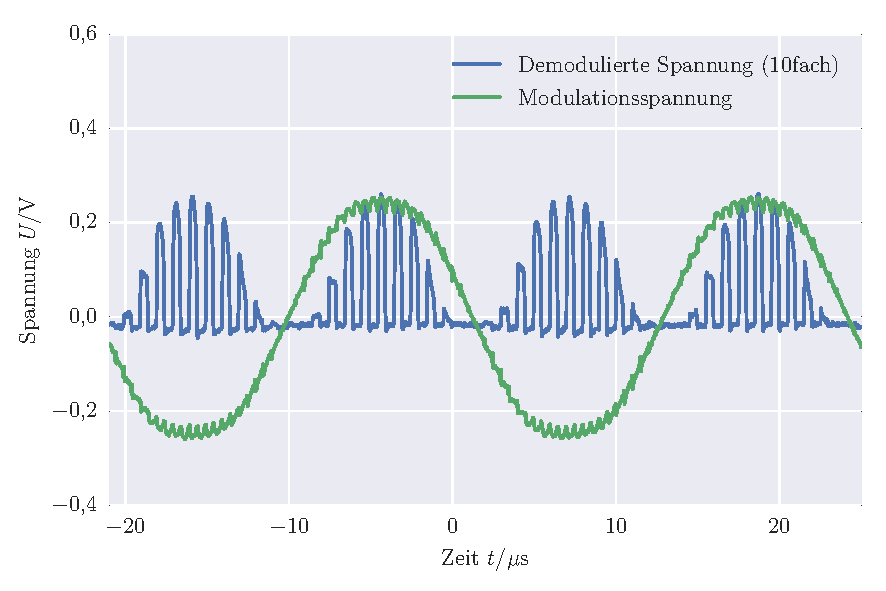
\includegraphics[scale=1]{../Grafiken/Amplituden_Modulation_Diode_Demodulation_Gleichrichter.pdf}
\caption{Spannung die in der Demodulationsschaltung mit Diode nach ebendieser abgegriffen wurde.
	Zu erkennen ist, dass die unteren Halbwellen der modulierten Eingangsspannung durch die Diode
	unterdrückt werden. Der Vergleich mit der Modulationsspannung zeigt das die übrig gebliebenen 
	oberen Halbwellen ihre Amplitude mit der Modulationsfrequenz verändern.   
	\label{fig:amplituden_modulation_diode_demodulation_gleichrichter}}
\end{figure}
\FloatBarrier